% =============================================================================
% SECTION - ÉNERGIE POTENTIELLE
% Chapitre 3 - Énergie et travail
% =============================================================================

\section{Énergie potentielle}
\label{sec:energie_potentielle}
% =============================================================================

Dans la section précédente, nous avons vu que le travail effectué par une force modifie l'énergie cinétique d'un objet. Mais que se passe-t-il lorsqu'on soulève un objet à vitesse constante? Le travail effectué ne se retrouve pas sous forme d'énergie cinétique... Où va-t-il?

\subsection{Le concept d'énergie potentielle}

Prenons l'exemple d'un conteneur qu'on soulève avec une grue. On effectue un travail sur le conteneur en le soulevant, mais sa vitesse reste essentiellement constante. L'énergie transférée au conteneur est en quelque sorte \textbf{emmagasinée} : elle sera éventuellement retransformée en énergie cinétique si le conteneur se met à tomber.

\begin{definition}[title=Énergie potentielle]
L'\textbf{énergie potentielle} est l'énergie qu'un système possède en raison de sa \textbf{position} ou de sa \textbf{configuration}. C'est une énergie « en réserve » qui peut être convertie en énergie cinétique.

L'énergie potentielle confère à un système la \textbf{capacité d'accomplir un travail}, tout comme l'énergie cinétique.
\end{definition}

\begin{remarque}[title=Exemples d'énergie potentielle dans le contexte maritime]
\begin{itemize}
    \item L'eau retenue derrière un barrage possède de l'énergie potentielle gravitationnelle qui peut faire tourner des turbines
    \item Un ancre soulevée au-dessus du fond marin possède de l'énergie potentielle
    \item Les ressorts des amortisseurs de choc sur les bollards stockent de l'énergie potentielle élastique
    \item Un conteneur suspendu par une grue possède de l'énergie potentielle qui pourrait causer des dommages s'il tombait
\end{itemize}
\end{remarque}

\subsection{Énergie potentielle gravitationnelle}

Lorsqu'un objet est soulevé près de la surface de la Terre, il acquiert de l'énergie potentielle gravitationnelle. Cette énergie dépend de la hauteur de l'objet.

\begin{definition}[title=Énergie potentielle gravitationnelle]
L'énergie potentielle gravitationnelle d'un objet de masse $m$ situé à une hauteur $y$ au-dessus d'un niveau de référence est :

\begin{equationimportante}
\begin{equation}
U_g = mgy
\label{eq:energie_potentielle_grav}
\end{equation}
\end{equationimportante}

où :
\begin{itemize}
    \item $m$ est la masse de l'objet (en kg)
    \item $g = \SI{9,8}{m/s^2}$ est l'accélération gravitationnelle
    \item $y$ est la hauteur au-dessus du niveau de référence (en m)
\end{itemize}

L'unité est le \textbf{joule} (J).
\end{definition}

\begin{attention}[title=Choix du niveau de référence]
Le niveau de référence ($y = 0$) peut être choisi \textbf{arbitrairement}. En pratique, on choisit généralement :
\begin{itemize}
    \item Le point le plus bas du problème
    \item Le sol ou le niveau de l'eau
    \item Tout autre niveau qui simplifie les calculs
\end{itemize}

\textbf{Important :} Seules les \textbf{variations} d'énergie potentielle ont une signification physique, pas la valeur absolue. Le choix du niveau de référence n'affecte pas le résultat final d'un problème.
\end{attention}

\begin{center}
\begin{tikzpicture}[scale=0.7]
    % Axe y
    \draw[axe, thick, ->] (0,0) -- (0,7) node[above] {$y$};
    
    % Niveau de référence
    \fill[blue!10] (-1,0) rectangle (8,0.3);
    \draw[very thick, blue] (-1,0) -- (8,0);
    \node[blue, right] at (8,0) {Niveau de référence ($y = 0$, $U_g = 0$)};
    
    % Objet en hauteur
    \fill[orange] (3,5) circle (8pt);
    \node[right] at (3.5,5) {Objet de masse $m$};
    
    % Hauteur
    \draw[<->, thick, red] (1,0) -- (1,5) node[midway, left] {$y$};
    
    % Énergie potentielle
    \node[right] at (4,5) {$U_g = mgy$};
    
    % Flèche gravité
    \draw[vecteur vert] (3,5) -- (3,3.5) node[right] {$\vect{F}_g$};
    
    % Annotations
    \node[below] at (3.5,-1) {L'axe $y$ pointe vers le haut};
\end{tikzpicture}
\end{center}

\begin{remarque}[title=Lien entre travail et énergie potentielle gravitationnelle]
Le travail effectué par la gravité et la variation d'énergie potentielle sont reliés par :
\[ W_g = -\Delta U_g = -(U_{g,f} - U_{g,i}) = U_{g,i} - U_{g,f} \]

En d'autres mots : quand un objet \textbf{descend}, il \textbf{perd} de l'énergie potentielle et la gravité effectue un travail \textbf{positif}. Quand un objet \textbf{monte}, il \textbf{gagne} de l'énergie potentielle et la gravité effectue un travail \textbf{négatif}.
\end{remarque}

\begin{exemple}{Énergie potentielle d'une ancre}{}
Une ancre de masse $m = \SI{2000}{kg}$ est suspendue à \SI{15}{m} au-dessus du fond marin. Calculez son énergie potentielle gravitationnelle en prenant le fond marin comme niveau de référence.

\begin{center}
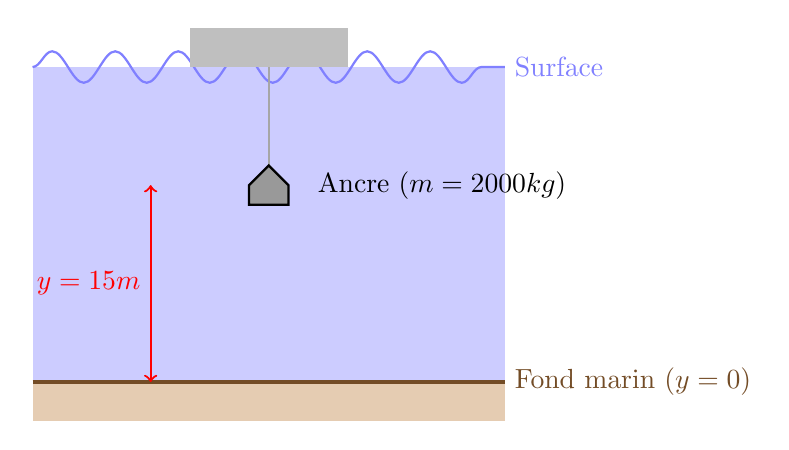
\begin{tikzpicture}[scale=0.5]
    % Eau
    \fill[blue!20] (-2,0) rectangle (10,8);
    
    % Fond marin
    \fill[brown!40] (-2,-1) rectangle (10,0);
    \draw[very thick, brown!60!black] (-2,0) -- (10,0);
    \node[brown!60!black, right] at (10,0) {Fond marin ($y = 0$)};
    
    % Surface
    \draw[blue!50, thick, decorate, decoration={snake, amplitude=2mm, segment length=8mm}] (-2,8) -- (10,8);
    \node[blue!50, right] at (10,8) {Surface};
    
    % Navire (simplifié)
    \fill[gray!50] (2,8) -- (6,8) -- (6,9) -- (2,9) -- cycle;
    
    % Chaîne
    \draw[thick, gray!70] (4,8) -- (4,5);
    
    % Ancre
    \fill[gray!80] (3.5,4.5) -- (4.5,4.5) -- (4.5,5) -- (4,5.5) -- (3.5,5) -- cycle;
    \draw[thick] (3.5,4.5) -- (4.5,4.5) -- (4.5,5) -- (4,5.5) -- (3.5,5) -- cycle;
    \node[right] at (5,5) {Ancre ($m = \SI{2000}{kg}$)};
    
    % Hauteur
    \draw[<->, thick, red] (1,0) -- (1,5) node[midway, left] {$y = \SI{15}{m}$};
\end{tikzpicture}
\end{center}

\textbf{Énergie potentielle gravitationnelle :}
\[ U_g = mgy = \SI{2000}{kg} \times \SI{9,8}{m/s^2} \times \SI{15}{m} \]
\[ U_g = \SI{294000}{J} = \SI{294}{kJ} \]

Cette énergie serait convertie en énergie cinétique (et éventuellement en chaleur et son) si l'ancre tombait jusqu'au fond.
\end{exemple}

\begin{pratiqueautonome}
Un conteneur de masse $m = \SI{12000}{kg}$ est chargé sur un navire. Il passe d'une hauteur de \SI{2}{m} (sur le quai) à une hauteur de \SI{8}{m} (dans la cale).

\begin{enumerate}[label=\alph*)]
    \item En prenant le niveau du quai comme référence, calculez l'énergie potentielle initiale et finale du conteneur.
    \item Calculez la variation d'énergie potentielle $\Delta U_g$.
    \item Quel travail la grue a-t-elle dû effectuer contre la gravité pour soulever le conteneur?
\end{enumerate}

\espaceresolution[6cm]
\reponsepratique{a) $U_{g,i} = \SI{235200}{J}$, $U_{g,f} = \SI{940800}{J}$ \quad b) $\Delta U_g = +\SI{705600}{J}$ \quad c) $W_{\text{grue}} = +\SI{705600}{J}$ (au minimum, contre la gravité)}
\end{pratiqueautonome}

\subsection{Énergie potentielle élastique}

Les ressorts et autres éléments élastiques peuvent également stocker de l'énergie potentielle. Cette énergie dépend de la déformation du ressort par rapport à sa position d'équilibre.

\begin{definition}[title=Énergie potentielle élastique]
L'énergie potentielle élastique d'un ressort déformé de $x$ par rapport à sa position d'équilibre est :

\begin{equationimportante}
\begin{equation}
U_e = \frac{1}{2}kx^2
\label{eq:energie_potentielle_elastique}
\end{equation}
\end{equationimportante}

où :
\begin{itemize}
    \item $k$ est la constante de rappel du ressort (en N/m)
    \item $x$ est la déformation (compression ou étirement) par rapport à l'équilibre (en m)
\end{itemize}

L'unité est le \textbf{joule} (J).
\end{definition}

\begin{remarque}[title=Propriétés de l'énergie potentielle élastique]
\begin{itemize}
    \item $U_e$ est \textbf{toujours positive ou nulle} (car $x^2 \geq 0$)
    \item $U_e = 0$ uniquement lorsque le ressort est à sa position d'équilibre ($x = 0$)
    \item La même énergie est stockée pour une compression ou un étirement de même amplitude
\end{itemize}
\end{remarque}

\begin{center}
\begin{tikzpicture}[scale=0.8]
    % Position d'équilibre
    \draw[thick] (0,2) -- (0.5,2);
    \draw[decoration={coil, segment length=4mm, amplitude=3mm}, decorate, thick] (0.5,2) -- (3,2);
    \draw[thick] (3,2) -- (3.5,2);
    \fill[blue!50] (3.5,1.5) rectangle (4.5,2.5);
    \node[below] at (4,1.3) {Équilibre};
    \node[below] at (4,0.8) {$x = 0$, $U_e = 0$};
    
    % Ressort comprimé
    \draw[thick] (0,5) -- (0.5,5);
    \draw[decoration={coil, segment length=2.5mm, amplitude=3mm}, decorate, thick] (0.5,5) -- (2,5);
    \draw[thick] (2,5) -- (2.5,5);
    \fill[red!50] (2.5,4.5) rectangle (3.5,5.5);
    \draw[<->, thick] (3.5,4) -- (4.5,4) node[midway, below] {$x$};
    \node[below] at (3,3.5) {Comprimé};
    \node[below] at (3,3) {$U_e = \frac{1}{2}kx^2$};
    
    % Ressort étiré
    \draw[thick] (0,-1) -- (0.5,-1);
    \draw[decoration={coil, segment length=5.5mm, amplitude=3mm}, decorate, thick] (0.5,-1) -- (4,-1);
    \draw[thick] (4,-1) -- (4.5,-1);
    \fill[green!50] (4.5,-1.5) rectangle (5.5,-0.5);
    \draw[<->, thick] (3.5,-2) -- (5.5,-2) node[midway, below] {$x$};
    \node[below] at (5,-2.8) {Étiré};
    \node[below] at (5,-3.3) {$U_e = \frac{1}{2}kx^2$};
    
    % Mur
    \fill[pattern=north east lines] (-0.3,6) rectangle (0,3.5);
    \fill[pattern=north east lines] (-0.3,3) rectangle (0,0.5);
    \fill[pattern=north east lines] (-0.3,0) rectangle (0,-2);
\end{tikzpicture}
\end{center}

\begin{exemple}{Amortisseur de bollard}{}
Un bollard d'amarrage est équipé d'un système d'amortissement à ressort avec une constante $k = \SI{50000}{N/m}$. Lorsqu'un navire tire sur l'amarre, le ressort se comprime de $x = \SI{0,15}{m}$.

\textbf{Énergie potentielle élastique stockée :}
\[ U_e = \frac{1}{2}kx^2 = \frac{1}{2} \times \SI{50000}{N/m} \times (\SI{0,15}{m})^2 \]
\[ U_e = \frac{1}{2} \times 50000 \times 0,0225 = \SI{562,5}{J} \]

Cette énergie est restituée au navire lorsque la tension diminue, ce qui amortit les à-coups.
\end{exemple}

\begin{pratiqueautonome}
Un système de lancement de canot de sauvetage utilise un ressort de constante $k = \SI{8000}{N/m}$. Le ressort est comprimé de \SI{0,5}{m} avant le lancement.

\begin{enumerate}[label=\alph*)]
    \item Calculez l'énergie potentielle élastique stockée dans le ressort.
    \item Si toute cette énergie est transférée à un canot de \SI{200}{kg}, quelle sera sa vitesse de lancement?
\end{enumerate}

\espaceresolution[5cm]
\reponsepratique{a) $U_e = \frac{1}{2} \times 8000 \times 0,25 = \SI{1000}{J}$ \quad b) $v = \sqrt{2U_e/m} = \sqrt{2 \times 1000/200} = \SI{3,16}{m/s}$}
\end{pratiqueautonome}

\subsection{Lien entre travail et énergie potentielle}

Il existe une relation fondamentale entre le travail effectué par certaines forces et la variation d'énergie potentielle associée.

\begin{definition}[title=Relation travail -- énergie potentielle]
Pour les forces qui possèdent une énergie potentielle associée (comme la gravité et la force de rappel), le travail effectué par ces forces est égal à \textbf{moins} la variation d'énergie potentielle :

\begin{equationimportante}
\begin{equation}
W = -\Delta U = -(U_f - U_i) = U_i - U_f
\label{eq:travail_energie_potentielle}
\end{equation}
\end{equationimportante}
\end{definition}

\begin{remarque}[title=Interprétation]
Cette relation nous dit que :
\begin{itemize}
    \item Quand l'énergie potentielle \textbf{diminue} ($\Delta U < 0$), la force effectue un travail \textbf{positif} (elle « libère » de l'énergie)
    \item Quand l'énergie potentielle \textbf{augmente} ($\Delta U > 0$), la force effectue un travail \textbf{négatif} (elle « stocke » de l'énergie)
\end{itemize}

C'est exactement ce qu'on observe : un objet qui tombe perd de l'énergie potentielle gravitationnelle, et la gravité effectue un travail positif sur lui.
\end{remarque}

\begin{exemple}{Vérification de la relation pour la gravité}{}
Vérifions la relation $W_g = -\Delta U_g$ pour un conteneur de \SI{1000}{kg} qui descend de \SI{5}{m}.

\textbf{Méthode 1 -- Par le travail :}
\[ W_g = -mg\Delta y = -(\SI{1000}{kg})(\SI{9,8}{m/s^2})(-\SI{5}{m}) = +\SI{49000}{J} \]

\textbf{Méthode 2 -- Par l'énergie potentielle :}
\begin{align*}
U_{g,i} &= mgy_i = 1000 \times 9,8 \times 5 = \SI{49000}{J} \\
U_{g,f} &= mgy_f = 1000 \times 9,8 \times 0 = \SI{0}{J} \\
\Delta U_g &= U_{g,f} - U_{g,i} = 0 - 49000 = -\SI{49000}{J} \\
W_g &= -\Delta U_g = -(-49000) = +\SI{49000}{J} \checkmark
\end{align*}

Les deux méthodes donnent le même résultat, ce qui confirme la relation.
\end{exemple}
